\chapter{Implementation in Pabutools}\label{chap:3}
Theoretical statements, though necessary to establish proportionality and formal implications, do not enable empirical evaluation themselves. Software implementations of them are pivotal: they allow for benchmark performance on real-life datasets, provide reusable code for the other researches to build-up on and let us assess election rules in practice. In this thesis, we pay particular attention to the practical side of the computational social choice theory.
\section{Overview of the repository}
Pabutools~\cite{Pabutools} is an open source Python library which provides a complete set of tools to work with participatory budgeting instances, that is:
\begin{itemize}
    \item a model layer with classes \emph{Project, Instance, Ballot, Profile}, allowing the user to handle PB instances of different kinds such as approval-based and cardinal-based elections.
    \item implementations of numerous election rules, such as many variants of the Method of Equal Shares, Utilitarian Greedy, Phragmén and many more.
    \item an analysis subpackage with axiom implementations and corresponding tests, for axioms such as Priceability or Justified Representation.
    \item full support for the instances taken from the Pabulib~\cite{Pabulib} library.
    \item seamless hooks for adding new rules or axioms.
\end{itemize}
\begin{figure}[H]         
  \centering              
  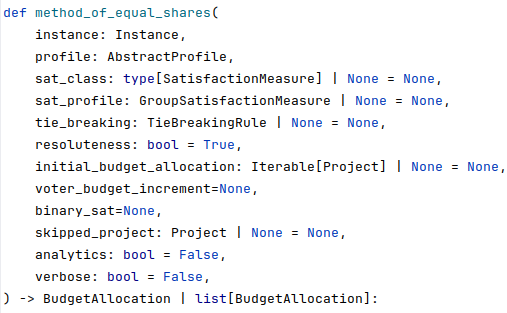
\includegraphics[width=0.7\textwidth]{figures/MES_method_pabutools.png}
  \caption{Function header for MES in Pabutools, showcasing most important data structures used throughout Pabutools.}
  \label{fig:myplot}
\end{figure}
It is important to note that election rules may choose different outcomes depending on the \emph{SatisfactionMeasure} they were called with. \emph{SatisfactionMeasure} is an abstract class representing a satisfaction measure for a given ballot. Two of the most important satisfaction measures for us are \emph{cost satisfaction measure} and \emph{additive cardinal satisfaction measure}.
\section{Integration of additive Stable-Priceability}
Implementation for finding and verifying priceable and stable priceable allocations already existed in the Pabutools library as part of analysis subpackage. However, it only supported profiles of \emph{AbstractApprovalProfile}. We extend it more broadly to \emph{AbstractProfile}, as it is the superclass of both \emph{ApprovalProfile} and \emph{CardinalProfile}. \emph{OrdinalProfile} is not supported though and it is explicitly rejected in the implementation. If the open-source community decides to provide a mapping from ordinal ballots to cardinal ballots, the ordinal setting could also be then served by this implementation.
\begin{figure}[H]         
  \centering              
  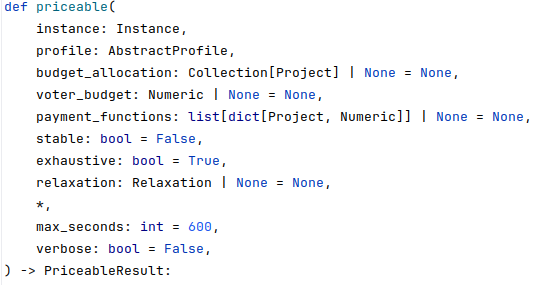
\includegraphics[width=0.7\textwidth]{figures/Priceable_function_header.png}
  \caption{Function header for stable priceability in Pabutools.}
  \label{fig:myplot}
\end{figure}
The above method either finds or verifies simple priceable allocations when \emph{stable := False} or stable-priceable allocations otherwise. Our work consisted only of updating the notion of stable-priceability, therefore implementation for simple priceability remained unchanged, except for updating the notion of supporting a candidate to cardinal ballots.

In order to reuse the same code for approval and cardinal ballots, minor changes to ballot classes were also added: functions \emph{utility} and \emph{supports}. For abstract ballot, the default implementation raises \emph{NotImplementedError}.
\begin{figure}[H]
  \centering
  \begin{minipage}{0.4\textwidth}
    \centering
    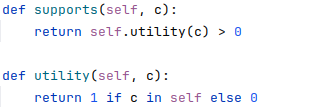
\includegraphics[width=\linewidth]{figures/cardinal_utility.png}
    \caption{Mentioned functions in CardinalBallot class.}
    \label{fig:img1}
  \end{minipage}\hfill
  \begin{minipage}{0.4\textwidth}
    \centering
    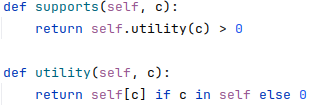
\includegraphics[width=\linewidth]{figures/approval_utility.png}
    \caption{Mentioned functions in ApprovalBallot class.}
    \label{fig:img2}
  \end{minipage}
\end{figure}

Additionally, stability relaxations have been adjusted to account for new definition of stable priceability. Though now they work with any additive utilities, their behaviour has only been studied and tested in the case of binary utilities. Extending and empirically studying these relaxations for cardinal ballots remains future work; Pabutools is structured to support this exploration with minimal changes.
\section{Testing}
To ensure the correctness of the implementation and the theoretical soundness of the proposed extension, a set of tests was also added to the project. The Pabutools library already contained some test cases for approval-based implementation of the \emph{priceable} function. They consisted of a couple of small, very well-understood instances for which solutions are known from manual analysis and prior literature, often coming from examples from papers on the subject and from the website on the Method of Equal Shares~\cite{EqualSharesWebsite}.

A key part of the tests aim to verify, that the updated function does indeed reduce to previous, approval-only implementation, in order not to break existing analysis tools and provide backwards compatibility. Pre-existing tests are reused for this, as the solution is expected to be exactly the same. A test was also added to verify if the new implementation does imply core up-to-one.

Finally, a new set of tests based on deeply analysed cardinal-based instances are added, to verify implementation for slightly more complex scenarios. These instances, similar in spirit to original set of tests, provide strong arguments for the correctness of the new implementation.